\documentclass[11pt]{aghdpl}
% \documentclass[en,11pt]{aghdpl}  % praca w języku angielskim

% Lista wszystkich języków stanowiących języki pozycji bibliograficznych użytych w pracy.
% (Zgodnie z zasadami tworzenia bibliografii każda pozycja powinna zostać utworzona zgodnie z zasadami języka, w którym dana publikacja została napisana.)
\usepackage[english,polish]{babel}

% Użyj polskiego łamania wyrazów (zamiast domyślnego angielskiego).
\usepackage{polski}

\usepackage[utf8]{inputenc}

% dodatkowe pakiety

\usepackage{mathtools}
\usepackage{amsfonts}
\usepackage{amsmath}
\usepackage{amsthm}

% --- < bibliografia > ---

\usepackage[
style=numeric,
sorting=none,
%
% Zastosuj styl wpisu bibliograficznego właściwy językowi publikacji.
language=autobib,
autolang=other,
% Zapisuj datę dostępu do strony WWW w formacie RRRR-MM-DD.
urldate=edtf,
% Nie dodawaj numerów stron, na których występuje cytowanie.
backref=false,
% Podawaj ISBN.
isbn=true,
% Nie podawaj URL-i, o ile nie jest to konieczne.
url=false,
%
% Ustawienia związane z polskimi normami dla bibliografii.
maxbibnames=3,
% Jeżeli używamy BibTeXa:
backend=bibtex,
seconds=true
]{biblatex}

\usepackage{csquotes}
% Ponieważ `csquotes` nie posiada polskiego stylu, można skorzystać z mocno zbliżonego stylu chorwackiego.
\DeclareQuoteAlias{croatian}{polish}

\begin{filecontents}{bibliografia.bib}
@online{Bonding,
  author = {Stu Borman},
  title = {Spying On Bond Making In Solution},
  date = {2015-02-19},
  url = {http://cen.acs.org/articles/93/i8/Spying-Bond-Making-Solution.html},
  urldate = {2015-03-03},
  addendum= {All about dicyanoaurate, has links to papers.}
}
\end{filecontents}

\addbibresource{bibliografia.bib}

% Nie wyświetlaj wybranych pól.
%\AtEveryBibitem{\clearfield{note}}


% ------------------------
% --- < listingi > ---

% Użyj czcionki kroju Courier.
\usepackage{courier}

\usepackage{listings}
\lstloadlanguages{TeX}

\lstset{
	literate={ą}{{\k{a}}}1
           {ć}{{\'c}}1
           {ę}{{\k{e}}}1
           {ó}{{\'o}}1
           {ń}{{\'n}}1
           {ł}{{\l{}}}1
           {ś}{{\'s}}1
           {ź}{{\'z}}1
           {ż}{{\.z}}1
           {Ą}{{\k{A}}}1
           {Ć}{{\'C}}1
           {Ę}{{\k{E}}}1
           {Ó}{{\'O}}1
           {Ń}{{\'N}}1
           {Ł}{{\L{}}}1
           {Ś}{{\'S}}1
           {Ź}{{\'Z}}1
           {Ż}{{\.Z}}1,
	basicstyle=\footnotesize\ttfamily,
}

% ------------------------

\AtBeginDocument{
	\renewcommand{\tablename}{Tabela}
	\renewcommand{\figurename}{Rys.}
}

% ------------------------
% --- < tabele > ---

\usepackage{array}
\usepackage{tabularx}
\usepackage{multirow}
\usepackage{booktabs}
\usepackage{makecell}
\usepackage[flushleft]{threeparttable}

% defines the X column to use m (\parbox[c]) instead of p (`parbox[t]`)
\newcolumntype{C}[1]{>{\hsize=#1\hsize\centering\arraybackslash}X}


%---------------------------------------------------------------------------

\author{Piotr Jaromin}
\shortauthor{P. Jaromin}

%\titlePL{Przygotowanie bardzo długiej i pasjonującej pracy dyplomowej w~systemie~\LaTeX}
%\titleEN{Preparation of a very long and fascinating bachelor or master thesis in \LaTeX}

\titlePL{Aplikacja internetowa wyznaczająca ograniczenia prędkości na drogach na podstawie danych z OpenStreetMap}
\titleEN{Web application that determines speed limits on roads based on data from OpenStreetMap}


\shorttitlePL{Aplikacja internetowa wyznaczająca ograniczenia prędkości na drogach na podstawie danych z OpenStreetMap} % skrócona wersja tytułu jeśli jest bardzo długi
\shorttitleEN{Web application that determines speed limits on roads based on data from OpenStreetMap}

\thesistype{Praca dyplomowa magisterska}

\supervisor{dr inż. Grzegorz Rogus}

\degreeprogramme{Informatyka}

\date{2018}

\department{Katedra Informatyki Stosowanej}

\faculty{Wydział Elektrotechniki, Automatyki,\protect\\[-1mm] Informatyki i Inżynierii Biomedycznej}

\acknowledgements{Serdecznie dziękuję \dots tu ciąg dalszych podziękowań np. dla promotora, żony, sąsiada itp.}


\setlength{\cftsecnumwidth}{10mm}

%---------------------------------------------------------------------------
\setcounter{secnumdepth}{4}
\brokenpenalty=10000\relax

\begin{document}

\titlepages

% Ponowne zdefiniowanie stylu `plain`, aby usunąć numer strony z pierwszej strony spisu treści i poszczególnych rozdziałów.
\fancypagestyle{plain}
{
	% Usuń nagłówek i stopkę
	\fancyhf{}
	% Usuń linie.
	\renewcommand{\headrulewidth}{0pt}
	\renewcommand{\footrulewidth}{0pt}
}

\setcounter{tocdepth}{2}
\tableofcontents
\clearpage

\chapter{Wprowadzenie}
\label{cha:wprowadzenie}


\section{Wstęp}
\label{sec:wstep}

Bezpieczeństwo na drodze stanowi jedno z podstawowych celów stawianych zarówno przez budowniczych dróg, producentów samochodów ich użytkowników a także osób znajdujących się pobliżu. Aby zredukować liczbę wypadków, niezbędne jest uwzględnienie ogromnej liczby czynników wpływających na bezpieczeństwo na drogach. Należy wziąć pod uwagę warunki atmosferyczne występujące w danej okolicy, ukształtowanie terenu, roślinność która może niekorzystnie wpłynąć na widoczność, drzewa znajdujące się w pobliżu tras oraz samo oznakowanie dróg. Ważne są także pojazdy, które biorą udział w ruchu, funkcję jakie spełnia dana droga, ilość pasów ruchu i ich szerokość, liczba zakrętów i promień ich skrętu oraz typ nawierzchni, z której składa się jezdnia. Nie należy lekceważyć także statystyk dotyczących wypadków na danych odcinkach dróg. Na bezpieczeństwo na drogach wpływ mają również producenci pojazdów. Rozwijane przez nich inteligentne czujniki oraz systemy wspomagania jazdy mają kluczowe znaczenie w redukcji ryzyka popełnienia błędu przez człowieka.

W tabeli \ref{BiomechanicznaToleracja}. znajduje się zestawienie przedstawiające tolerancje biomechaniczną człowieka dla różnych typów pojazdów.

\newcommand{\source}[1]{\caption*{Source: {#1}} }

\begin{table}[ht]
\centering
\caption{Biomechaniczna tolerancja na wypadki}
\label{BiomechanicznaToleracja}
\begin{tabular}{| l | c |}
\hline
\textbf{Typ wypadku}                    & \textbf{Prędkość uderzenia} \\ \hline
samochód / pieszy / rowerzysta          & 20 - 30 km/h                                    \\ \hline
samochód / motocykl                     & 20 - 30 km/h                                    \\ \hline
samochód / drzewo lub słup              & 30 - 40 km/h                                    \\ \hline
samochód / samochód (zderzenie boczne)  & 50 km/h                                         \\ \hline
samochód / samochód (zderzenie czołowe) & 70 km/h   \\ \hline
\end{tabular}
\source{Na podstawie Austroroads 2005}
\end{table}

Z tabeli \ref{BiomechanicznaToleracja}. odczytać można, że najbardziej podatni na zagrożenia w ruchu drogowym są piesi, rowerzyści i motocykliści. Oczywiście są to uśrednione dane. Ryzyko poważnych obrażeń, a nawet śmierci, w niektórych przypadkach może wystąpić przy jeszcze mniejszych prędkościach.

\newpage


W ''Raport o stanie bezpieczeństwa ruchu drogowego dla dróg krajowych w zarządzie GDDKiA'' opublikowanym na stronie Generalnej Dyrekcji Dróg Krajowych i Autostrad, znajduje się zestawienie liczby wypadków drogowych i ich skutków, w latach 2007 - 2016.

\begin{figure}[h]
\caption{wypadki drogowe i ich skutki}
\label{wypadkiSkutki}
\centering
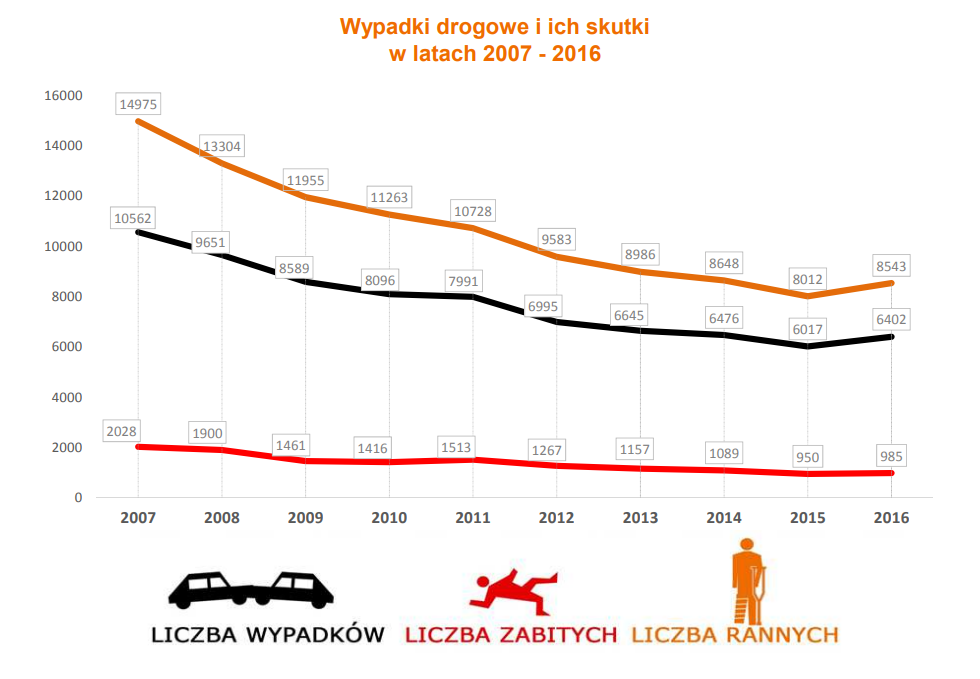
\includegraphics[width=1\textwidth]{picture1}
\source{Raport o stanie bezpieczeństwa ruchu drogowego dla dróg krajowych w zarządzie GDDKiA.}
\end{figure}

Z Rys. \ref{wypadkiSkutki} odczytać można, że liczba wypadków, z jednym wyjątkiem (z roku 2016) nieustannie maleje. W 2007 roku miało miejsce 10562 wypadków, w których liczba zabitych wyniosła 2028 osób, natomiast rannych było 14975. W porównaniu z 2016 został odnotowany spadek o ok. 40 \%. Niewątpliwie jest to ogromny sukces, jednak liczba ta dalej jest zatrważająco wysoka.


\section{Cele pracy}
\label{sec:celePracy}

Głównym celem niniejszej pracy dyplomowej było stworzenie inteligentnego systemu, mającego za zadanie predykcję dopuszczalnych prędkości w ruchu drogowym. Ponadto zostały opracowane modele i narzędzia pozwalające na obliczenie prędkości ma drogach. Rozwiązanie bazuje na metodach automatycznego wnioskowania, modelach matematycznych i informacjach geoprzestrzennych. Dzięki temu, możliwe było wyznaczenie optymalnego rozwiązania dla złożonego, wielokryterialnego problemu, w którym kluczowe znaczenie miało bezpieczeństwo uczestników ruchu drogowego, przy zachowaniu maksymalnej przepustowości infrastruktury drogowej.

Algorytm predykcji dopuszczalnych prędkości w ruchu drogowym wykorzystuje następujące informacje

\begin{itemize}
\item \textbf{pojedyncze poziome zakręty} - zostały podzielone na trzy grupy, według długości promienia skrętu:
 \begin{itemize}
 	\item \textbf{mały promień skrętu} - o maksymalnej długości promienia 300m
 	\item \textbf{średni promień skrętu} - o długości promienia powyżej 300m i poniżej 600m
 	\item \textbf{duży promień skrętu} - o długości promienia powyżej 600m
 \end{itemize}
\item \textbf{pobliże szkół i miejsc zabaw} - w takich przypadkach prędkość musiała zostać dobrana, aby kierowca bez przeszkód mógł zatrzymać się, nie powodując zagrożenia dla zdrowia i życia osób niepełnoletnich. Należy mieć na uwadze fakt, że zachowanie małoletnich osób często jest nieobliczalne. Nigdy nie wiadomo kiedy mogą pojawić się na drodze
\item \textbf{pobliże sklepów i miejsc kultów religijnych} - dostosowanie prędkości do większego niż zwykle ruchu pieszych jak i pojazdów mechanicznych.
\item \textbf{pobliże przystanków autobusowych i tramwajowych} - zdarzają się szczególne sytuacje, gdy pasażerowie komunikacji zbiorowej, bez uprzedniego upewnienia się, biegną  do już odjeżdżającego autobusu czy tramwaju. W takim przypadku szczególnie ważne jest dostosowanie prędkości, żeby kierowca mógł bez przeszkód, odpowiednio wcześniej, zareagować na taką ewentualność
\item \textbf{przejścia dla pieszych} - w sytuacjach jak powyżej, z tą różnicą, że zamiast na autobus, przebiegają na ''późnym zielonym'' lub czasem już czerwonym. Do takich sytuacji najczęściej dochodzi w miastach, gdzie tempo życia jest bardzo duże. Należy pamiętać, że ok. 25\% wypadków na przejściach z sygnalizacją spowodowane jest wtargnięciem pieszego na czerwonym świetle
\item \textbf{ilość pasów ruchu} - prędkość jest większa na kilku pasmowej drodze, w porównaniu z jednopasmową
\item \textbf{typ nawierzchni} - jest to bardzo ważny czynnik, ponieważ pojazdy mechaniczne, poruszając się z nieodpowiednią prędkością po nieprzystosowanej do tego nawierzchni, np. żwirowej, bardzo szybko ulegają kosztownym uszkodzeniom
\item \textbf{typ drogi} - w skład których wchodzą autostrady, drogi osiedlowe, ekspresowe, główne itp.
\item \textbf{zmiana prędkości między poszczególnymi strefami ograniczeń prędkości} - płynna jazda jest znacznie mniej ryzykowna niż nagła zmiana prędkości pojazdu. Dlatego w sytuacjach, gdy na drodzę znajduje się np. przejście dla pieszych, należy stopniowo ustawiać coraz to niższe wartości znaków sygnalizujących ograniczenie prędkości
\item \textbf{przejazdy kolejowe} - są zarówno strzeżone jak i niestrzeżone. W obu przypadkach należy zachować szczególną ostrożność, dlatego też prędkość musi być odpowiednio niższa. Trzeba mieć na uwadze, że przez dużą masę pojazdów szynowych, wypadki kolejowe należą do jednych z najbardziej śmiercionośnych.
\end{itemize}

Oprócz danych pobranych z OpenStreetMap, program posiada możliwość manualnego, przez zwykłego użytkownika, definiowania obiektów i przeszkód na drodze. Jest to szczególnie istotne, gdyż nie wszystkie dane umieszczone są w OSM.


Kluczową kwestią działanie algorytmu są również miejsca, w których powinien umieszczać znaki ograniczenia prędkości. Kierowca odpowiednio wcześniej musi zostać poinformowany o przeszkodzie na drodze, żeby mieć wystarczającą ilość czasu na reakcję. Dla przykładu, niedopuszczalna jest sytuacja, podczas której kierowca podróżując z szybkością 90 km/h, natrafia na znak informujący o znajdującym się za nim przejściu dla pieszych. Prawidłowo działający algorytm, powinien informować o potrzebie stopniowej redukcji prędkości, poprzez umieszczanie znaków ograniczeń prędkości o coraz to mniejszych wartościach. Dzięki temu możliwe jest zapewnienie płynność jazdy, przy zachowaniu odpowiedniego bezpieczeństwa.


%Raport o stanie bezpieczeństwa ruchu drogowego dla dróg krajowych w zarządzenie GDDKiA



\section{Wykorzystane technologie}
\label{sec:wykorzystaneTechnologie}
	Cała aplikacja bazuje na dynamicznej stronie internetowej. W tym celu został wykorzystany stos technologiczny, bazujący na javascripcie, jakim jest MEAN stack. Miałem kilka powodów, dla którym wybrałem te konkretne technologie. Pierwszym jest rosnąca popularność tego stosu. Coraz więcej firm przekonuje się do tej technologii, więc popyt na programistów z tego zakresu rośnie z roku na rok. Drugim powodem jest fakt, że można go uruchomić na prawie każdym urządzeniu czy platformie, dzięki czemu jest zapewniona duża przenośność kodu. Dodatkowo MEAN stack idealnie nadaje się do prostych, skalowalnych aplikacji webowych, w których nacisk kładziony jest na wymianę danych w czasie rzeczywistym na wielu urządzeniach.

	Back-end aplikacji został napisany w Node.js. Jego głównym zadaniem jest połączenie  się z mLabem w celu pobrania, zapisu, edycji i usuwania danych. Ponadto komunikuje się również z frontendem, po to, aby przekazywać pobrane dane.  Dodatkowo, w celu zmniejszenia objętości kodu i tym samym zwiększenia jego czytelności, został użyty framework Express.js.

	Za zarządzanie front-endem odpowiedzialny jest angular w wersji 5. Na nim została uruchomiona biblioteka Leaflet. Umożliwia ona wyświetlanie interaktywnej mapy, którą zasilić można różnymi typami danych, np. w formacie GeoJson. Dzięki niej, użytkownik zyskał możliwość wprowadzania swoich danych, przeglądania już istniejących czy zasięgnięcia informacji o dozwolonych prędkościach na danych odcinkach dróg. Kolejną,  istotną funkcjonalnością biblioteki Leaflet jest możliwość zarządzania wyświetlanymi obiektami. W prosty sposób można ukryć wszystkie dane, wyświetlać tylko drogi, tylko ograniczenia prędkości lub różne kombinację danych, które nas interesują.

\section{Przegląd literatury}
\label{sec:przegladLiteratury}

Han(2009) podaje przykład, jak zmiana prędkości wpływa na bezpieczeństwo i płynność jazdy. Jeśli kierowca napotka zbyt wiele stref prędkości z obrębie krótkiego odcinka drogi lub zbyt wiele zmian ograniczeń prędkości w sąsiedztwie danej strefy, to wtedy może poczuć dezorientację. Zwraca uwagę, jak ważne jest rozmieszczenie odpowiednich znaków, dla zredukowania poziomu stresu kierowcy.

Nama(2016) przedstawia jak kierowcy dostosowują prędkość w sytuacji gdy znajdują się na górzystej, nieregularnej drodze. Średnia wariancja prędkości w takim terenie wynosi ok. 55\%. Spowodowane jest to połączeniem cech geometrycznych zarówno poziomych jak i pionowych. Kierowcy na potrzeby bezpieczeństwa, w przypadku poziomych zakrętów, zmniejszają prędkość. Dodatkowym czynnikiem jest także ciągłe, zmieniające się nachylenie terenu. Uwzględnić należy również fakt, że zakręty znajdujące się na szczycie, wyglądają na znacznie bardziej niebezpieczne niż są w rzeczywistości. Wszystkie te czynniki w niekorzystny sposób wpływają na utrzymywanie stałej prędkości. Tabela \ref{predkosciPromienKrzywizny}. przedstawia średnią prędkość pojazdów w zależności od promienia krzywizny zakrętu, jego długości oraz nachylenia.


\begin{table}[ht]
\centering
\caption{Średnie prędkości pojazdów w zależności od promienia krzywizny, długości oraz nachylenia}
\label{predkosciPromienKrzywizny}
\begin{tabular}{| l | l | l | l | }
\hline
\textbf{promień krzywizny (m)} & \textbf{nachylenie (\%)} & \textbf{długość zakrętu (\%)} & \textbf{średnia prędkość (km/h)} \\ \hline
50 & 4 & 74 & 48.9\\ \hline
100 & 2 & 139 & 47.8\\ \hline
100 & -6 & 33 & 56.2\\ \hline
100 & 6 & 33 & 49.9\\ \hline
150 & -6 & 31 & 49.8\\ \hline
150 & -4 & 64 & 54.3\\ \hline
150 & 2 & 32 & 54.7\\ \hline
150 & 4 & 43 & 52.1\\ \hline
200 & -4 & 56 & 54.2\\ \hline
200 & -2 & 27 & 59.6\\ \hline
200 & 2 & 205 & 45.8\\ \hline
200 & 4 & 10 & 60.9\\ \hline
200 & 6 & 102 & 50.1\\ \hline
300 & -6 & 73 & 58.2\\ \hline
300 & 2 & 74 & 52.6\\ \hline

\end{tabular}
\source{Na podstawie Expanded Operating Speed Model}
\end{table}

W tabeli \ref{predkosciPromienKrzywizny} znalazły się dane z obserwacji na drodze, na której ograniczenie prędkości wynosiło 50 km/h. Zauważyć można, że w 45\% prędkość była wyższa niż  dopuszczalna.

Forbes(2012) wspomina o relacji pomiędzy prędkością, a ryzykiem wypadku dla prędkości pomiędzy 25 km/h a 120 km/h. Gdy średnia prędkość ruchu jest zmniejszona, liczba wypadków i  poziom niebezpieczeństwa spowodowania urazów prawie zawsze maleje. Gdy średnia prędkość ruchu wzrasta, liczba wypadków i poziom niebezpieczeństwa spowodowania urazów przeważnie rośnie. Relacja między średnią prędkością a ryzykiem wypadków może być adekwatnie opisana według poniższego modelu:

\begin{equation}
CMF = (V_a / V_b)^X
\end{equation}
gdzie
\begin{eqwhere}[2cm]
	\item[$CMF$] Współczynnik modyfikacji wypadku
	\item[$V_a$] średnia prędkość przed warunkiem
	\item[$V_b$] średnia prędkość po warunkiem
	\item[$X$] \begin{itemize}
		3.6 dla częstotliwości wypadków, w których pojawiły się ofiary śmiertelne

		2.0 dla częstotliwości wypadków, w których nie było ofiar śmiertelnych

		1.0 dla częstotliwości gdzie uszkodzeniu uległy tylko pojazdy

		4.5 dla ofiar śmiertelnych

		2.7 dla których poszkodowani ponieśli tylko obrażenia ciała
	\end{itemize}

\end{eqwhere}
Porównuje także ograniczenia prędkości dla poszczególnych obszarów znajdujących się w USA. Ich wynik znajduje się w tabeli \ref{ograniczeniaStany}.

\begin{table}[ht]
\centering
\caption{Ograniczenia prędkości w różnych stanach}
\label{ograniczeniaStany}
\begin{tabular}{|c|c|c|}
\hline
\textbf{Stan}                    & \textbf{Prędkość} & \textbf{Obszar} \\ \hline
\multirow{5}{*}{Delaware}   & 40 km/h & dowolna dzielnica biznesowa \\ \cline{2-3}
& 40 km/h & dowolna dzielnica mieszkalna \\ \cline{2-3}
& 30 km/h & wszystkie strefach szkolnych \\ \cline{2-3}
& 80 km/h & dwupasmowa jezdnia \\ \cline{2-3}
& 90 km/h & czteropasmowa jezdnia \\ \hline

\multirow{6}{*}{Minneasota}   & 15 km/h & alejki \\ \cline{2-3}
& 50 km/h & ulice dzielnic miejskich \\ \cline{2-3}
& 110 km/h & wiejskie autostrady międzystanowe \\ \cline{2-3}
& 105 km/h & miejskie autostrady międzystanowe \\ \cline{2-3}
& 105 km/h & drogi ekspresowe \\ \cline{2-3}
& 90 km/h & pozostałe drogi \\ \hline

\multirow{5}{*}{Oregon}   & 25 km/h & alejki, wąskie uliczki mieszkalne  \\ \cline{2-3}
& 30 km/h & dzielnice biznesowe, strefy szkolne \\ \cline{2-3}
& 40 km/h & dzielnice mieszkalne, parki publiczne, brzegi oceanu \\ \cline{2-3}
& 90 km/h & wiejskie autostrady, ciężarówki na międzystanowych autostradach \\ \cline{2-3}
& 105 km/h & pojazdy pasażerskie, lekkie ciężarówki na międzystanowych autostradach\\ \hline
\end{tabular}
\source{Na podstawie Methods and Practices for Setting Speed Limits: An Informational Report}
\end{table}


Han(2009) zwraca uwagę, jak pora dnia wpływa na ruch na drodzę. W godzinach porannych, gdy osoby pracujące jadą do pracy, osoby nieletnie do szkół oraz w godzinach popołudniowych, gdy wracają do domów. Obserwowany jest wzmożony ruch na drogach. Więcej pojazdów na drodze, oznacza większe korki, a co za tym idzie, zmniejszenie rzeczywistej prędkości. Natomiast w pozostałych porach dnia, gdy ruch jest mniejszy, możliwe jest szybsze poruszanie się po drodze. C. Han opisuje także jak prawidłowo ustawiać znaki drogowe. Oznakowanie powinno być umieszczone w każdym odpowiednim punkcie wzdłuż drogi, np. wokół potencjalnych punktów konfliktowych, zwężeniach i rozwidleniach dróg, zmianie ich nawierzchni itp. Powtórzenia znaków, najlepiej żeby były w odległości 1000m na autostradach. W obszarach miejskich, rekomendowana odległość to 400-500 m.

Jurewicz(2014) wskazuje bezpośrednią relację pomiędzy prędkością a ryzykiem wypadku. W sytuacji gdy prędkość jest zmniejszana,  liczba wypadków i rannych spada w 85 procentach przypadków. Gdy prędkość jest zwiększana, liczba wypadków i rannych wzrasta w 71 procentach przypadków. Największym dowodem na to są tak zwane badania 'przed i po'. W latach 1980 ograniczenie prędkości dla wiejskich i zewnętrznych autostrad w metropolii zostało zwiększone ze 100 km/h do 110 km/h, ale zostało  z powrotem zredukowane do 100 km/h z powodu obaw o bezpieczeństwo. Badanie 'przed, w trakcie i po' zostało prowadzone na przestrzeni 2,5 roku. W sytuacji, gdy ograniczenie prędkości zostało zwiększone do 110 km/h, wskaźnik ofiar wypadków wzrósł o prawie 25\%. Gdy prędkość ponownie została zmniejszona do 100 km/h wskaźnik zmalał o prawie 20\%.

Vadeby i Frosman (2018) przeprowadzili badania na temat, jak nowe ograniczenia prędkości wpłynęły na bezpieczeństwo. Dla przykładu, gdy na wiejskich drogach została zmniejszona wartość dozwolonej prędkości z 90 km/h do 80 km/h, zauważono spadek liczby wypadków śmiertelnych o 14 w skali roku. Nie zauważono natomiast żadnych znaczących zmian dla liczby poważnych obrażeń ciała. Na autostradzie, po zwiększeniu dozwolonej prędkości do 120 km/h, zanotowano wzrost wypadków, w których doszło do poważnych obrażeń. Nie odnotowano natomiast znaczącej zmiany względem ofiar śmiertelnych. Wzrost liczby poważnych obrażeń ciała wystąpił na wszystkich rodzajach autostrad, jednak największy wzrost został zauważony na wąskich autostradach o szerokości 21.5 m. Dla dwupasmowych jezdni, po zmniejszeniu prędkości ze 110 do 100 km/h, doszło do zmniejszenia liczby wypadków z poważnymi obrażeniami ciała o 16 w skali roku. Vadeby i Frosman (2018) wskazują także na fakt, iż wzrost dozwolonej prędkości o 10 km/h spowodował średni wzrost prędkości pojazdów mechanicznych o ok. 2-3 km/h, a zmniejszenie dozwolonej prędkości o 10 km/h, spowodował zmniejszenie średniej prędkości pojazdów o 3 km/h.

Soriguera i inni (2017) przeprowadzili badanie, które wykazało, jak mała wartość ograniczenia prędkości wpływa na ruch uliczny. Jako rezultat, uzyskali następujące wyniki.

\begin{itemize}
\item Dla ograniczenia prędkości do 80 km/h, maksymalna przepustowość może wynieść 1972 samochodów na godzinę na jednym pasie ruchu, dla szerokiego zakresu zajętości jezdni (17.6 - 25.8\%) i średniej prędkości wahającej się między 51 a 73 km/h
\item Dla ograniczenia prędkości do 60 km/h, maksymalna przepustowość nie uległa dużej zmianie, wyniosła 1956 pojazdów na godzinę na jednym pasie ruchu. Zajętość jezdni utrzymywała się na wysokim poziomie 24.4 - 25.8\%.
\item Dla ograniczenia prędkości do 40 km/h, maksymalna przepustowość nieznacznie zmalała, do poziomu 1942 samochodów na godzinę na jednym pasie ruchu. Natomiast znacznie wzrosła zajętość jedni, wynosiła 32.0 - 34.7\%.
\end{itemize}

Z powyższych wyników, można dojść do dwóch wniosków. Pierwszy jest taki, że zmniejszenie prędkości skutkuje znacznym zwiększeniem poziomu zajętości jezdni w warunkach swobodnego przepływu. W skrócie, zmniejszenie prędkości pozwala osiągnąć stabilny, wysoki poziom zajętości jezdni, zapobiegając tym samym różnym wypadkom i utrzymywaniem dużej akumulacji pojazdów na drodze. Drugi wniosek jest taki, że dla małej prędkości, jaką jest 40 km/h, średnia prędkość przepływu pojazdów, wynosząca 1942 pojazdów/h/pas, może zostać podtrzymana przez dłuższy okres. W praktyce oznacza to znaczne zmniejszenie prawdopodobieństwa wystąpienia korków na drodze.

\section{Układ pracy}
\label{sec:ukladPracy}

Praca składa się z 5 rozdziałów.

\begin{itemize}
\item Pierwszy z nich składa się ze wstępu, celów pracy, wykorzystanych technologii oraz przeglądu literatury.
\item W drugin rozdziale zawarto opracowanie teoretyczne poszczególnych części algorytmu. Przestawiono również ogólny schemat, sposób w jaki algorytm pobiera dane, skąd je bierze oraz jak je parsuje, przetwarza i wyświetla na stronie.
\item Trzeci rodział zawiera wyniki działania algorytmu dla poszczególnych jego składowych
\item W piątym rozdziale został umieszczony opis interfejsu użytkownika
\end{itemize}

\chapter{Interfejs użytkownika - TODO}
\label{cha:UI}
W niniejszym rozdziale skupię się na szczegółowym opisie interfejsu użytkownika. Zostaną przedstawione najważniejsze funkcję, które pomogą użytkownikowi w korzystaniu z programu. Omówinone zostaną poszczególne warstwy wyświetlone na mapie, przełączanie między nimi oraz tworzenie własnych warst, przedstawiających dodaną przez użytkownika informację. W pierwszej sekcji przedstawiony zostanie widok główny aplikacji wraz z dokładnym omówieniem. W dalszych częsciach tego rozdziału, opisane zostaną kolejne warstwy. Na końcu przedstawiony zostanie sposób, jak dodawać własne obiekty, żeby były widoczne na mapie.
\newpage
\section{Widok główny aplikacji}
\label{sec:mainView}

Rys. \ref{mainView}. przedstawia widok główny aplikacji. W lewym górnym rogu znajdują się dwa przyciski: ''+'' oraz ''-''. Umożliwiają one przybliżanie i oddalanie widoku mapy. W prawym górnym rogu znajduję się menu wyboru wyświetlanej warstwy. Szczegóły dostępne w rozdziale \ref{sec:layerMenu}. Ponadto, użytkownik posiada możliwość, za pomocą myszki, przesuwania obecnie wyświetlanej mapy w dowolnym kierunku. Mapa pobierana jest w czasie rzeczywistym ze strony OpenStreetMap.

\begin{figure}[h]
\caption{Widok główny aplikacji}
\label{mainView}
\centering
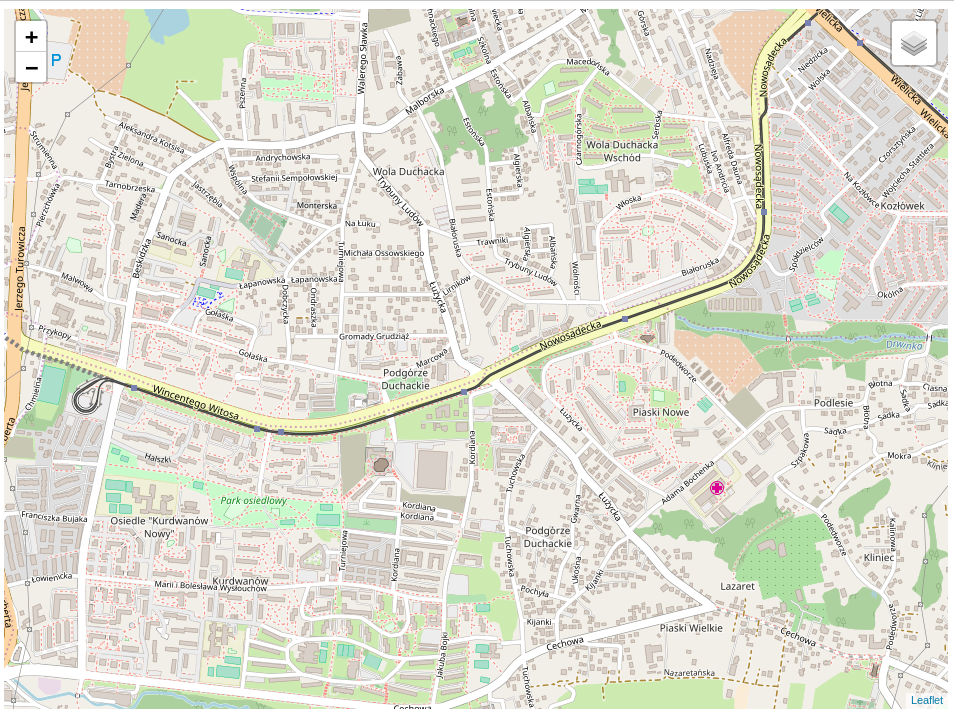
\includegraphics[width=1.1\textwidth]{mainScreen}
\end{figure}

\newpage

\section{Menu wyboru warstw}
\label{sec:layerMenu}

Rys. \ref{sec:mainLayerView}. przedstawia menu wyboru warstw. Dostępny jest dopiero po najechaniu kursorem myszki. Umozliwia wyświetlanie na mapie elementów, które użytkownik w danej chwili potrzebuje. 

\begin{figure}[h]
\caption{Menu wyboru warstw}
\label{sec:mainLayerView}
\centering
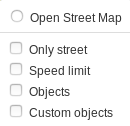
\includegraphics[width=0.4\textwidth]{layerMenu}
\end{figure}

Menu wyboru warst, Rys. \ref{sec:mainLayerView}, składa się z pięciu elementów:
\begin{itemize}
\item \textbf{Open Street Map} - domyślna warstwa, służąca do wyświetlania głównej mapy.
\item \textbf{Only street} - służy do zaznaczania na mapie, wszystkich dostępnych ulic. Więcej szczegółów znajduje się w rozdziale \ref{sec:onlyStreet}
\item \textbf{Speed limit} - najważniejsza warstwa, przedstawiajaca dopuszczalne prędkości na drogach. Więcej szczegółów znajduje się w rozdziale \ref{sec:speedLimit}
\item \textbf{Objects} - wyświetla obiekty istotne dla algorytmu obliczajacego predkość pojazdów. W ich skład wchodzą np. przystanki autobusowe i tramwajowe, szkoły, kościoły, place zabaw itp. Więcej szczegółów znajduje się w rozdziale \ref{sec:objects}
\item \textbf{Custom objects} - wyświetla dane wprowadzone przez wszystkich użytkowników aplikacji. Więcej szczegółów znajduje się w rozdziale \ref{sec:customObjects}
\end{itemize}

Istotną funkcjonalnością jest możliwość wyświetlania dowolnych kombinacji warstw. Użytkownik może zaznaczyć dowolną liczbę widoków, które zostaną wyswietlone na głównej mapie.

\newpage
\section{Widok zaznaczonych ulic}
\label{sec:onlyStreet}

Rys. \ref{sec:onlyStreetMap} przedstawia mapę, na której zaznaczone są poszczególne odcinki dróg. Reprezentowane są przez niebieskie linie łamane, przebiegającą przez sam jej środek. Zostały uzglednione różnego rodzaju klasy dróg, takie jak: 
\begin{itemize}
\item autostrady
\item drogi ekspresowe
\item drogi główne ruchu przyspieszonego
\item drogi główne
\item drogi zbiorcze
\item drogi lokalne
\item drogi dojazdowe
\end{itemize}

\begin{figure}[h]
\caption{Widok zaznaczonych ulic}
\label{sec:onlyStreetMap}
\centering
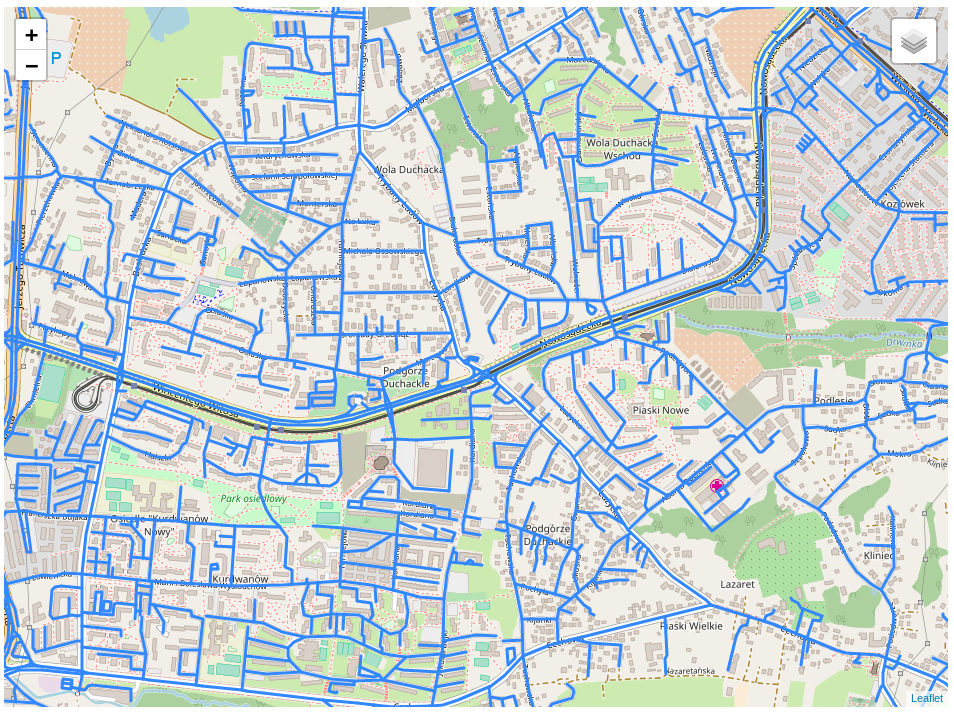
\includegraphics[width=1.03\textwidth]{onlyStreet}
\end{figure}

\newpage
\section{Widok dopuszczalnych ograniczeń prędkości}
\label{sec:speedLimit}


Na mapie z Rys. \ref{sec:speedLimitMap}, zostały umieszczone ograniczenia prędkości dla każdego odcinka drogi. Do wyznaczania tych ograniczeń, algorytm uwzględnił szereg czynników, które zostały opisane w późniejszych rozdziałach. Dla lepszej wizualizacji wyznaczonych danych, do wykonania Rys. \ref{sec:speedLimitMap}., został włączony także widok zaznaczonych ulic, opisany w rozdziale \ref{sec:onlyStreet}.

\begin{figure}[h]
\caption{Widok dopuszczalnych ograniczeń prędkości}
\label{sec:speedLimitMap}
\centering
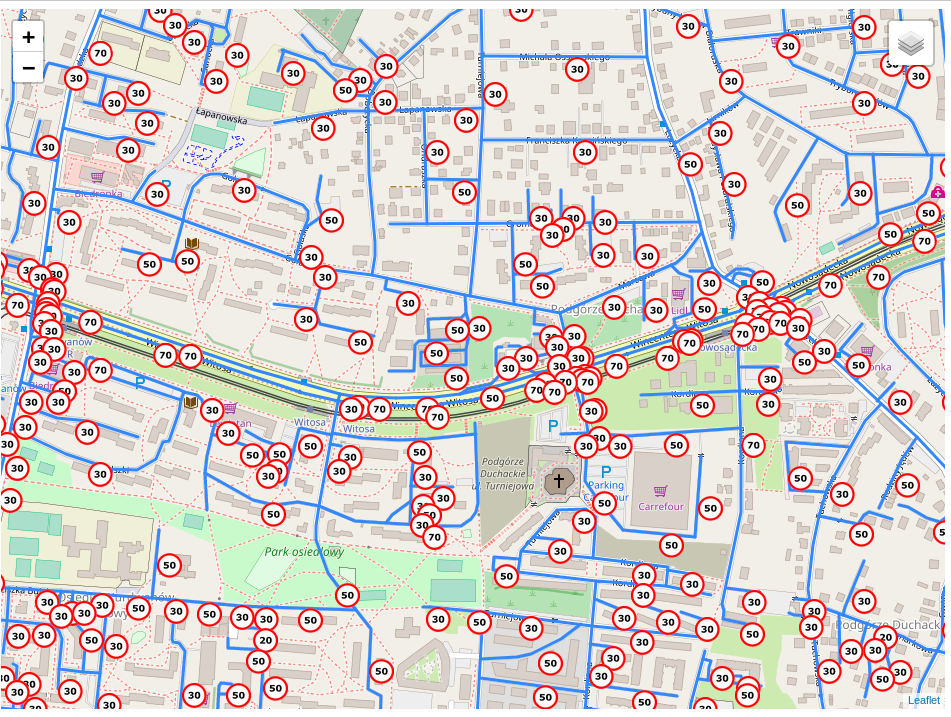
\includegraphics[width=1.03\textwidth]{speedLimit}
\end{figure}

\newpage
\section{Widok istotnych obiektów pobranych z OSM}
\label{sec:objects}

Rys. \ref{sec:objectsMap} przedstawia istotne, z puktu widzenia algorytmu, obiekty pobrane z OpenStreetMap. W ich skład wchodzą:
\begin{itemize}
\item przedszkola i szkoły
\item przystanki autobusowe i tramwajowe
\item przejścia dla pieszczych
\item sklepy i miejsca kultu religijnego
\item place zabaw
\end{itemize}

\begin{figure}[h]
\caption{Widok istotnych obiektów pobranych z OSM}
\label{sec:objectsMap}
\centering
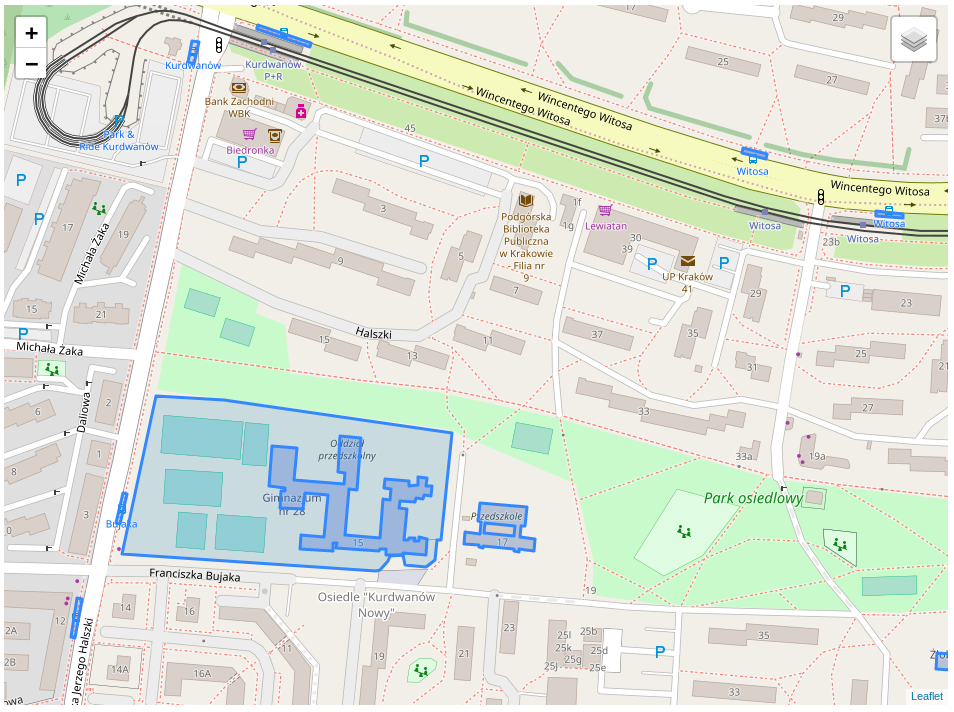
\includegraphics[width=1.03\textwidth]{objects}
\end{figure}

\newpage
\section{Widok obiektów zdefiniowanych przez użytkownika}
\label{sec:customObjects}

\newpage
\section{Dodawanie własnych obiektów}
\label{sec:addedCustomObjects}
\chapter{Harmonogram}
\label{cha:harmonogram}


\section{Harnomogram}
\label{sec:harmonogram}

\begin{table}[ht]
\centering
\caption{Harmonogram}
\label{Harmonogram}
\begin{tabular}{| p{12cm} | c |}
\hline
\textbf{Co?}                    & \textbf{Kiedy?} \\ \hline

Wstęp dokumentacji, aplikacja internetowa wyświetlająca dopuszczalne prędkości na mapie & 16.03.2018 \\ \hline

odpowiednie umieszczenie znaków & 23.03.2018 \\ \hline
pobliże szkół
pobliże sklepow i miejsc kultów
pobliże przystanków
pobliże przejścia dla pieszych 
przejazdy kolejnowe & 30.03.2018 \\ \hline

tunele i mosty
ilość pasów ruchu
typ nawierzchni
typ drogi & 06.04.2018 \\ \hline

historia wypadków & 13.04.2018 \\ \hline

płynna zmiana prędkości & 20.04.2018 \\ \hline

Zakręty & 27.04.2018 \\ \hline

Koncowa wersja aplikacji & 04.05.2018 \\ \hline

Końcowa wersja dokumentacji & 01.06.2018 \\ \hline
\end{tabular}
\end{table}




% itd.
% \appendix
% \include{dodatekA}
% \include{dodatekB}
% itd.



\printbibliography

\end{document}
